\emph{This chapter lays out the theoretical background of this thesis by first introducing the general concepts of a high-level language cirtual machine (HLL-VM) like the Java Virtual Machine (JVM) and then going on to more specific features of the GraalVM. In the following the next abstraction layer the Truffle API is explained before coming to the explicit project Graal.Js which uses Truffle. The last section evolves around the ECMAScript parts of the topic with a brief glance at the current state of modules and what the proposal tries to achieve.}

\section{HLL-VMs}
\subsection{HLL-VM groundwork}
Generally speaking a high-level language virtual machine is an abstraction layer relieving the programmer from several tasks with the main feature being platform independent development. When starting to discuss the platform independence it is foremost important to note why programs are usually platform bound.\\
Every computer employs some kind of an instruction set architecture (ISA) and an operating system (OS). Every developped program is bound to these two technologies. If a program is developed for a particular pair of ISA/OS it has to be ported to run on a machine with a different pair of ISA/OS. The problem arising with that is huge support overhead since now every ported version has to receive different kinds of updates. It is thus highly impractical to enforce such a development environment for every application program. By developing a high-level language virtual machine this task is posed upon the development of the VM only and all other application programs being developped don't have to focus on platform dependency resulting in a more lean development process. How is the VM doing this particular task?\\
High-level language virtual machines enhanced the concept of early VMs like P-code by using virtual instruction set architectures (V-ISA) encompassing code and metadata, like data structures and resource-related information, independently of platforms. The code is simpley interpreted the metadata loaded and thus turned into a machine-dependent version by the virtual machines provided emulator. This alone already stands out as a huge accomplishment but HLL-VMs come with even more features.\\
In today's computer landscape the highest risk comes from untrusted software run on machines. The HLL-VM, especially the JVM,  provides a metaphoric sandbox in which the untrusted application can run without making the rest of the system outside of the VM vulnerable. But although it amplifies security there are loopholes to bypass said security measures especially when untrusted software is given explicit permission to go outside of the VM provided resources. So running untrusted software is still not advised but made more secure so with a HLL-VM. As said before security is not the only feature HLL-VMs serve. Making code robust is another one.\\
Especially when it comes to large-scale software systems robust software is key. Here the good fit of the object-oriented model and the platform independence make HLL-VMs the top technology in the field. How much a HLL-VM supports robustness is of course depending on the used VM but on the example of the JVM strong type-checking and garbage collection which will be explained later lift a lot of beverage off the programmer's shoulder making the programmer concentrate on the mere implementation and thus making the programmer produce more robust code.\\
Other merits of HLL-VMs come from technologies like dynamic linking saving network bandwidth or profiling for performance.\cite{Smith}\\
As the start of this subsection already stated a HLL-VM is an abstraction layer with a lot of features making a programmer's life considerably easier. This comes with some costs especially with performance. This cost is then highly reduced by certain techniques like the forementioned profiling. With the groundwork laid out the next section discusses certain features of the JVM.

\subsection{The JVM}
The Java Virtual Machine is as its name states developed around the language Java. Java is a general-purpose, object-oriented language with strong static types aimed as a production language. Since one language target is simplicity details of machine representation are omitted and not accessable through the language. Further safety measures have been made like auomatic storage management and checked array access. The Java sourcecode is usually compiled ahead of time (AOT) to the Java bytecode which is then run on the JVM. Ahead of time compilation means that the programmed sourcecode gets compiled into a machine specific executable form. This form is in the case of Java Java bytecode, i.e. a class-file.\cite{Gosling}\par As stated before the JVM is the virtual sandbox environment in which an AOT-compiled java program, java bytecode, is executed. The JVM, like an actual machine, has an instruction set and access to various memory areas. With this in mind a JVM can also be directly implemented as a CPU or in various other direct ways. From knowing what the JVM is, the next paragraph dives deeper into the topic and explains how the JVM is constructed with the help of figure \ref{fig:jvm}.\\
As already explained the JVM executes Java bytecode which can be in the form of *.class-files. Before the thesis dives into the structure one note has to be made: The JVM is usually delivered as a Java Runtime Environment (JRE) or Java Development Kit (JDK). These include besides the Java Virtual Machine also the Java Application Programming Interface (API) classes. These are not directly part of the JVM but play a vital role in the simplification process for programming that is undertaken by the Java project. Coming to the execution the first substructure to mention is the Class Loader Environment.\\
\begin{figure}
	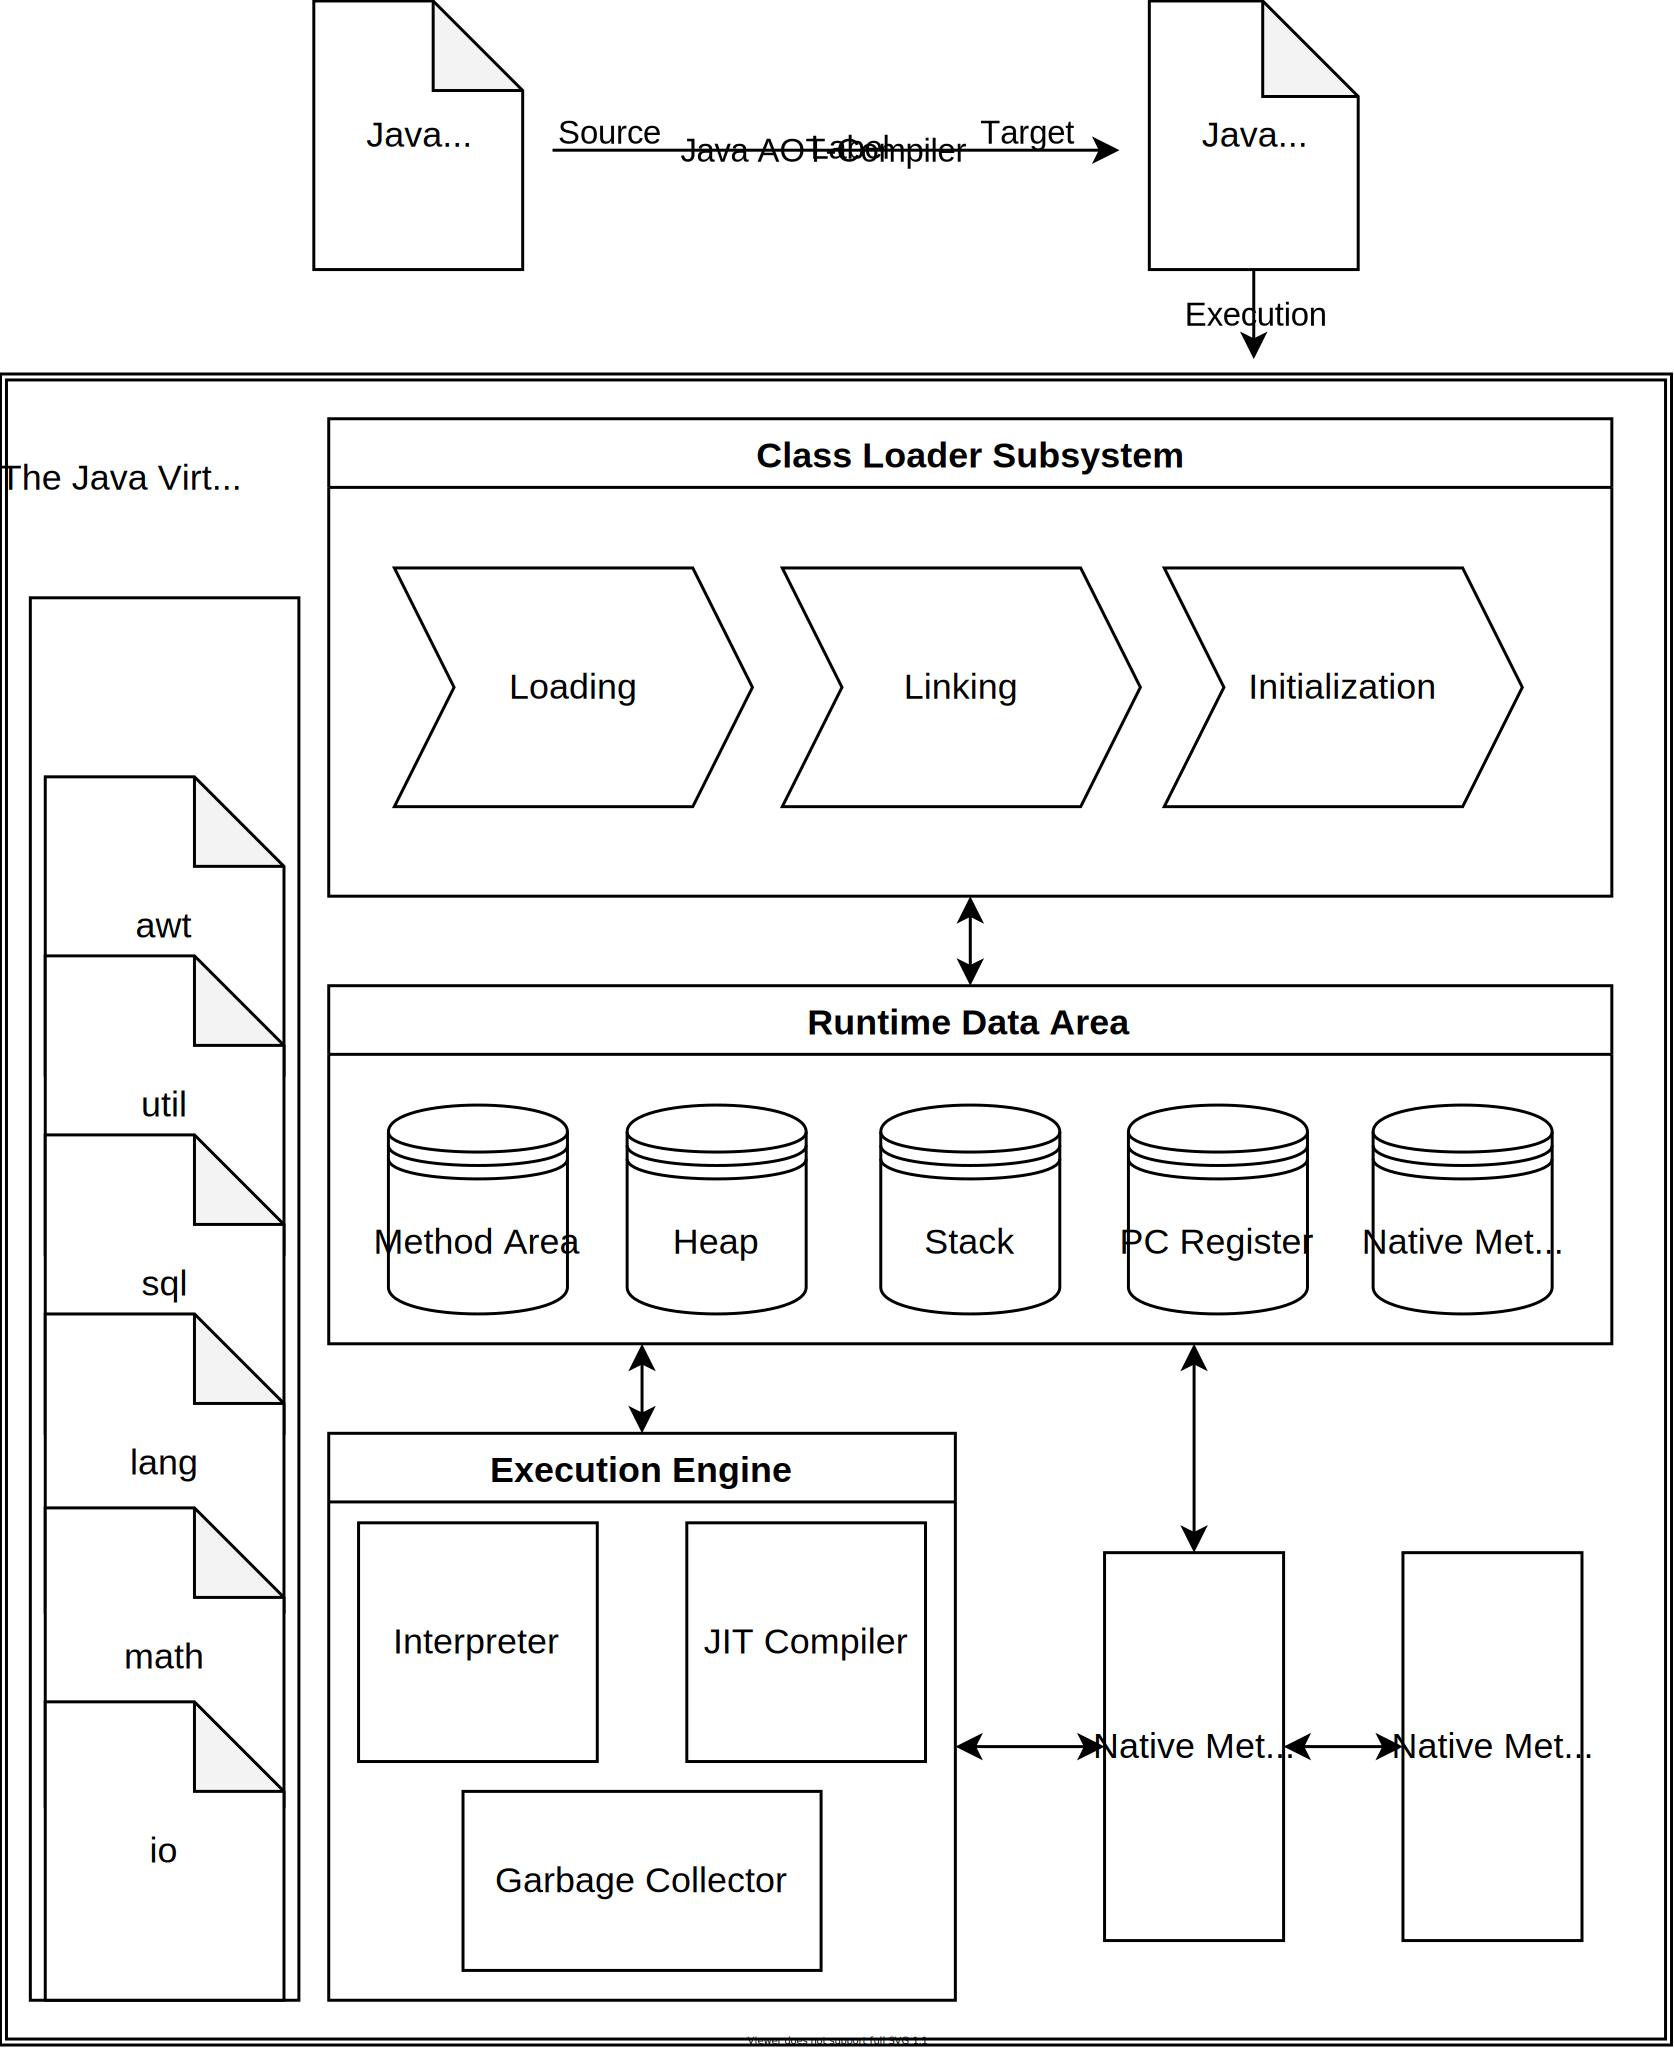
\includegraphics[scale=0.2]{../figures/JVM.png}
	\caption{The Java Virtual Machine simplified structure}
	\label{fig:jvm}
\end{figure}
When talking about the JVM the mentioning of classes and interfaces is inevitable.
In further parts the distinction between class and interface is abbreviated as class.
Multiple causes for class creation exist. The class to be created can be referenced by the constant pool of another class or a class' method can be invoked via reflection.\\
The creation at the start of a program works via loading the initial class and initializing it and furthermore invoking the specified method \emph{static void main(args[])}. The complete execution is driven by this method which, as soon as the program has more than this specific method and starting class, causes loading, linking and initialization of additional classes and invoking additional methods. How do the three steps, loading, linking and initialization work? The next paragraph talks about the beginning of a class creation and loading.\\
When creating a class in execution the JVM transforms the implementation-independent bytecode into an implementation-specific internal representation of the class. The algorithm is executed step by step meaning that a class has to be completely loaded before linking can be started and it has to be verified and prepared to the full extant before initialization.\\
The loading is started by the class loader which can be the JVM bootstrap loader or a user-defined one. Before the JVM starts the class loader it checks whether the pair binary class name and class loader already exist in which case the class already exists thus eliminating the necessity of class creation. If creation proves necessary the class loader has to find the class' bytecode representation on the specific platform, usually a file with the class' name in a hierarchical filesystem. After finding, if not a specific error is thrown, the JVM parses the bytecode, which in turn might not be valid resulting in different kinds of errors. Optional superclasses may also be resolved. After these steps the pair of loader and class are saved by the JVM. Loading usually concerns the class itself however linking concerns the whole ecosystem of the respective class. \\
The JVM links a class by preparing the class, superclasses, element type in cas of array classes and resolving all symbolic references which as it is a recursive algorithm includes loading and linking these as well. The two strategies are an eager algorithm, meaning immediate loading and linking, or loading and linking in a lazy way meaning resources are only loaded and linked when they are about to be used.

\cite{Lindholm}


\section{GraalVM}

\section{Truffle API}

\section{Graal.Js}

\section{ECMAScript modules}
\subsection{Current State}

\subsection{Proposal: Module blocks}